\documentclass{article}
\usepackage[italian]{babel}
\usepackage[tmargin=2cm,rmargin=1.5in,lmargin=1.5in,margin=0.85in,bmargin=2cm,footskip=.2in]{geometry}
\usepackage{siunitx}
\sisetup{separate-uncertainty=true, per-mode=fraction, parse-numbers=true}
\usepackage{caption}
\usepackage[T1]{fontenc}
\usepackage{bookmark}
\usepackage{mathcomp}
\usepackage{graphicx}
\usepackage{multicol}
\usepackage{booktabs}
\usepackage{amsmath,amsfonts,amsthm,amssymb,mathtools}
\hypersetup{
	pdftitle={Relazione pendolo fisico},
	colorlinks=true, linkcolor=doc!90,
	bookmarksnumbered=true,
	bookmarksopen=true
}
\usepackage{blindtext}
\usepackage{wrapfig}
\usepackage{listings}
\usepackage{xcolor}
\usepackage{float}
\usepackage{amsmath}
\usepackage{amssymb}
\usepackage{tikz}
\usepackage{titling}
\renewcommand\maketitlehooka{\null\mbox{}\vfill}
\renewcommand\maketitlehookd{\vfill\null}
\usepackage{multirow}
\usepackage{biblatex}
\definecolor{codegreen}{rgb}{0,0.6,0}
\definecolor{codegray}{rgb}{0.5,0.5,0.5}
\definecolor{codepurple}{rgb}{0.58,0,0.82}
\definecolor{backcolour}{rgb}{0.95,0.95,0.92}
\definecolor{doc}{rgb}{0,0,0}
\lstdefinestyle{code}{
    backgroundcolor=\color{backcolour},   
    commentstyle=\color{codegreen},
    keywordstyle=\color{magenta},
    numberstyle=\tiny\color{codegray},
    stringstyle=\color{codepurple},
    basicstyle=\ttfamily\footnotesize,
    breakatwhitespace=false,         
    breaklines=true,                 
    captionpos=b,                    
    keepspaces=true,                                     
    showspaces=false,                
    showstringspaces=false,
    showtabs=false,                  
    tabsize=2,
    inputencoding=ansinew,
    extendedchars=true,
    numbers=left,                    
    numbersep=5pt
}

\lstset{style=code}
\usepackage[varbb]{newpxmath}
\usepackage{circuitikz}
\captionsetup{labelfont={bf, sc}}
\title{Lunghezza Focale}
\author{Giosuè Aiello}
\date{\today}

\begin{document}
	\begin{titlingpage}
    \begin{center}
        \vspace*{60pt} % Spazio dall'inizio della pagina

        {\Huge \textbf{\textsc{Lunghezza Focale}}} % Titolo in maiuscoletto
        \vspace{30pt} % Spazio dopo il titolo

        {\huge{Giosuè Aiello}} % Autore in corsivo e un po' più piccolo
        \vspace{20pt} % Spazio dopo l'autore

        {\large \today} % Data
    \end{center}
    
    \vfill % Riempie lo spazio verticale rimanente
\end{titlingpage}

\pagebreak
%-------------------------------------------------------------------------------------------------
%---------------------------------------------------------------------------------------------------------------------------------------------------------------------------------------------------------------------------------------------------------------------
\section{Scopo dell'esperienza}
L’obiettivo dell’esperienza consiste nella misura della lunghezza focale di una lente divergente.

%-------------------------------------------------------------------------------------------------
%---------------------------------------------------------------------------------------------------------------------------------------------------------------------------------------------------------------------------------------------------------------------
\section{Premesse teoriche}
	Una lente è un dispositivo ottico in grado di far concentrare o disperdere i raggi luminosi. \\
	\noindent Una lente divergente (\textbf{Figura~\ref{fig:l.d}}) è un tipo di lente che, per l'appunto, fa divergere i raggi luminosi che la attraversano, facendo in modo che questi provengano da un punto dietro la lente stessa: siccome forma esclusivamente \emph{immagini virtuali} necessitiamo di una lente convergente con un potere diottrico maggiore in modulo rispetto a quello delle lente divergente. \\
	Per calcolare la lunghezza focale della lente divergente si utilizza la legge dei punti coniugati (nel caso di lenti sottili), che risulta essere
	\begin{equation}
		\frac{1}{p} + \frac{1}{q} = \frac{1}{f}
		\label{lens_maker}	
	\end{equation}
	dove $p$ e $q$ rappresentano, rispettivamente, la distanza fra la lente e lo schermo (quando essa non è a fuoco) e la distanza fra la lente e lo schermo con l'immagine a fuoco. \\
	Un fatto interessante è che la~(\ref{lens_maker}) mostra come per determinare la lunghezza focale $f$ sia necessario conoscere sia $p$ che $q$, ma se
	\begin{equation}
		\frac{1}{\hat{p}} \ll \frac{\sigma_q}{q^2} \, \implies \hat{p} \gg \frac{\hat{q}^2}{\sigma_q^2}
	\end{equation}
	allora si potrebbe trascurare il termine $\frac{1}{p}$ e misurare solamente $\frac{1}{q}$ (effettuando quindi una sola misura).
\\\\
Non ostante la sintesi sia un elemento caraterizante per una spiegazione esaustiva trovo doveroso esplicare il funzionamento delle lenti convergenti e divergenti incentrando attenzione sulla loro manipolazione geometrica nei confronti dei raggi luminosi. Per cui:  
\subsection*{Lenti Divergenti}
Una lente divergente è una lente che disperde i raggi di luce che la attraversano. Questi raggi, dopo il passaggio attraverso la lente, si allontanano tra loro come se provenissero da un punto focale situato dietro la lente stessa. Le lenti divergenti sono caratterizzate da una forma più sottile al centro e più spessa ai bordi, e possiedono una potenza diottrica negativa, indicata con un segno meno \textbf{"-"}.

\vspace{0.5cm}

\begin{figure}[htbp]
	\begin{minipage}{0.55 \textwidth}
		\centering
		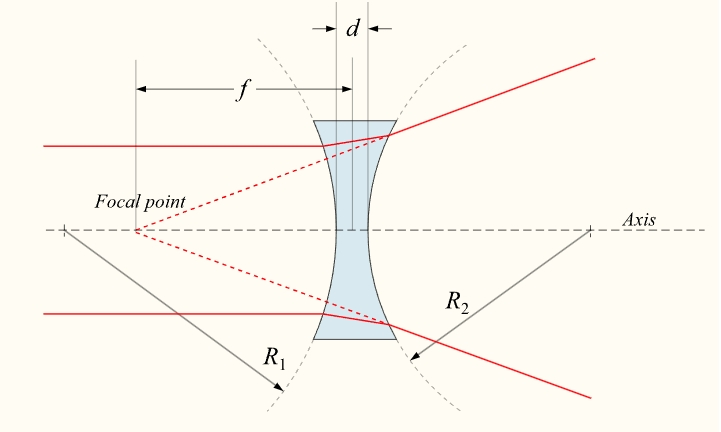
\includegraphics[width=\linewidth]{lente.divergente}
		\caption{Schematizazione di una lente divergente}	
		\label{fig:l.d}
	\end{minipage}
\hfill	
	\begin{minipage}{0.40 \textwidth}
		Nella \textbf{Figura~\ref{fig:l.d}} che troviamo qui a fianco è schematizzato il funzionamento di una  lente divergente, osserviamo quest'ultima che manipola i raggi di luce rossi: questi, entrando da sinistra, si disperdono allontanandosi dall'asse principale una volta attraversata la lente. Le superfici R1 e R2 definiscono i confini della lente, mentre il punto focale a sinistra segnala dove i raggi paralleli si incontrerebbero se prolungati idealmente. La lunghezza focale, denotata con 'f', è negativa, a indicare la divergenza dei raggi. La distanza 'd' è la misura tra i punti focali ai lati opposti della lente, e l'asse principale, segnato come 'Asse', si estende orizzontalmente attraverso il suo centro.
	\end{minipage}
	
\end{figure}

\pagebreak

\subsection*{Lenti Convergenti}
In questo stile: Una lente convergente è una lente che raccoglie i raggi di luce che la attraversano. Questi raggi, dopo il passaggio attraverso la lente, si avvicinano tra loro come se fossero diretti verso un punto focale situato davanti alla lente stessa. Le lenti convergenti sono caratterizzate da una forma più spessa al centro e più sottile ai bordi, e possiedono una potenza diottrica positiva, indicata con un segno più \textbf{"+"}.
\vspace{0.5cm}

\begin{figure}[htbp]
	\begin{minipage}{0.55 \textwidth}
		\centering
		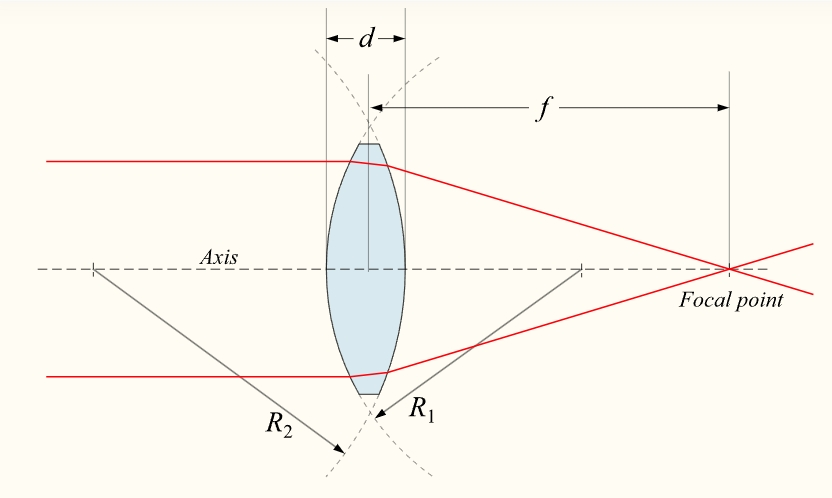
\includegraphics[width=\linewidth]{lente.convergente}
		\caption{Schematizazione di una lente convergente}	
		\label{fig:l.c}
	\end{minipage}
\hfill	
	\begin{minipage}{0.40 \textwidth}
		Nella \textbf{Figura~\ref{fig:l.c}} qui accanto, vediamo una lente biconvessa. Questa lente ha due superfici curve, \( R1 \) e \( R2 \), che rifrangono i raggi di luce e li fanno convergere in un punto focale. I raggi di luce entrano paralleli all'asse ottico della lente e, dopo aver attraversato la lente, convergono in un punto focale sullo stesso asse. La distanza tra il centro della lente e il punto focale è indicata con \( "f" \), che rappresenta la lunghezza focale della lente. Infine, la distanza \( "d" \) indica lo spessore della lente al centro.

	\end{minipage}
\end{figure}
%-------------------------------------------------------------------------------------------------
%---------------------------------------------------------------------------------------------------------------------------------------------------------------------------------------------------------------------------------------------------------------------

\section{Strumenti e materiali}

\textbf{Strumenti}

\begin{itemize}
    \item metro a nastro, con risoluzione $\pm 0.1 \si{\centi\meter}$
\end{itemize}

\textbf{Materiali}

\begin{itemize}
    \item banco ottico con sorgente luminosa
    \item lente di lunghezza focale ignota
    \item schermo
    \item cassetta di lenti convergenti o divergenti
\end{itemize}

\noindent ~\hrulefill 
%-------------------------------------------------------------------------------------------------
%---------------------------------------------------------------------------------------------------------------------------------------------------------------------------------------------------------------------------------------------------------------------
	
	\section{Descrizione delle misure}
Per semplificare la presa dei dati, la sorgente era coperta da un pezzo di plastica da cui era stato rimosso un triangolino: in questa maniera era più facile individuare se l'immagine era messa a fuoco siccome i bordi del triangolo si delineavano ancora più netti. Inizialmente ho verificato che la lente dal potere diottrico ignoto fosse divergente: questo è stato possibile prendendo la lente e ponendola davanti alla sorgente, osservando che non esisteva alcun punto in cui i raggi convergessero. Come spiegato nelle premesse teoriche, per misurare la lunghezza focale necessitiamo di una lente convergente: per questo ho considerato una lente con potere diottrico di +20 e abbiamo spostato lo schermo per mettere a fuoco l'immagine sullo schermo. A quel punto abbiamo posto la lente divergente fra lo schermo e la lente convergente e abbiamo misurato la distanza arbitraria p = -15 cm fra lo schermo e la lente. Successivamente abbiamo spostato lo schermo in modo da rimettere a fuoco l'immagine e abbiamo misurato la distanza q = 25 cm fra lo schermo e la lente. Iterando questo procedimento, abbiamo effettuato in totale 10 misurazioni. Come incertezza non abbiamo utilizzato la risoluzione dello strumento siccome non conoscevamo bene la posizione del centro della lente e non si riusciva a trovare il punto esatto di messa a fuoco, ma solamente un intervallo in cui l'immagine sullo schermo risultava essere a fuoco; dunque abbiamo deciso di utilizzare questo intervallo come incertezza di misura, che è stato stimato intorno a 0.5 cm.

	

\clearpage
%-------------------------------------------------------------------------------------------------
%---------------------------------------------------------------------------------------------------------------------------------------------------------------------------------------------------------------------------------------------------------------------

\section{Analisi dei dati}
Prima di addentrarci nel dettaglio della nostra analisi dei dati è doveroso dire che i calcoli presenti in questa relazione come lo stesso \textit{fit} delle misure sono stati fatti utilizzando \texttt{python} unito a funzioni come \texttt{curve\_fit} della libreria \texttt{scipy}.
\\
\begin{table}[htbp]
\begin{minipage}{0.55\textwidth}
\centering
\begin{tabular}{cc}
\toprule
p (cm) & q (cm) \\
\midrule
\midrule
$4.6 \pm 0.29$ & $6.1 \pm 0.50$ \\
$6.4 \pm 0.29$ & $9.8 \pm 0.64$ \\
$7.9 \pm 0.29$ & $14.9 \pm 0.81$ \\
$8.5 \pm 0.29$ & $14.6 \pm 0.80$ \\
$9.6 \pm 0.29$ & $19.5 \pm 0.96$ \\
$10.5 \pm 0.29$ & $22.8 \pm 1.08$ \\
$11.6 \pm 0.29$ & $28.3 \pm 1.26$ \\
$12.7 \pm 0.29$ & $44.1 \pm 1.74$ \\
$13.5 \pm 0.29$ & $49.4 \pm 1.90$ \\
$15.2 \pm 0.29$ & $66.8 \pm 2.43$ \\
\bottomrule
\end{tabular}
\caption{Misure sperimentali.}
\label{tab:misure_focale}
\end{minipage}
\hfill
\begin{minipage}{0.45\textwidth}
Nella \textbf{Tabella~\ref{tab:misure_focale}} La prima colonna rappresenta la distanza p tra la lente divergente e lo schermo quando l'immagine non è a fuoco, mentre la seconda colonna rappresenta la distanza q tra la lente divergente e lo schermo quando l'immagine è a fuoco. Le incertezze associate alle misure sono riportate accanto ai valori corrispondenti.
\end{minipage}
\end{table}
\\
I dati non soddisfano la condizione $\frac{1}{\hat{p}} \ll \frac{\sigma_q}{q^2}$ dunque non possiamo trascurare il termine $\frac{1}{p}$. Ad esempio, per il primo punto dati:
\begin{equation*}
\frac{1}{\hat{p}} = 0.1000 \quad \gg \quad \frac{\sigma_q}{q^2} = 0.0066
\end{equation*}
Il valore di $\frac{1}{\hat{p}}$ non è molto più piccolo del valore di $\frac{\sigma_q}{q^2}$, quindi la condizione non è soddisfatta.

Linearizziamo la~\eqref{lens_maker} ponendo $x = \frac{1}{q}$ e $y=\frac{1}{p}$ e si ottiene
\begin{equation}
y = mx + \frac{1}{f}
\end{equation}
e possiamo dunque effettuare un fit utilizzando come modello teorico una semplice retta che ha $m$ come coefficiente angolare e $\frac{1}{f}$ come intercetta con l'asse y. Tuttavia si osserva che gli errori sugli $x_i$ non sono trascurabili e quindi abbiamo utilizzato gli errori efficaci.

Riporto il grafico del fit:

\begin{figure}[htbp]
\begin{minipage}{0.55\textwidth}
\centering
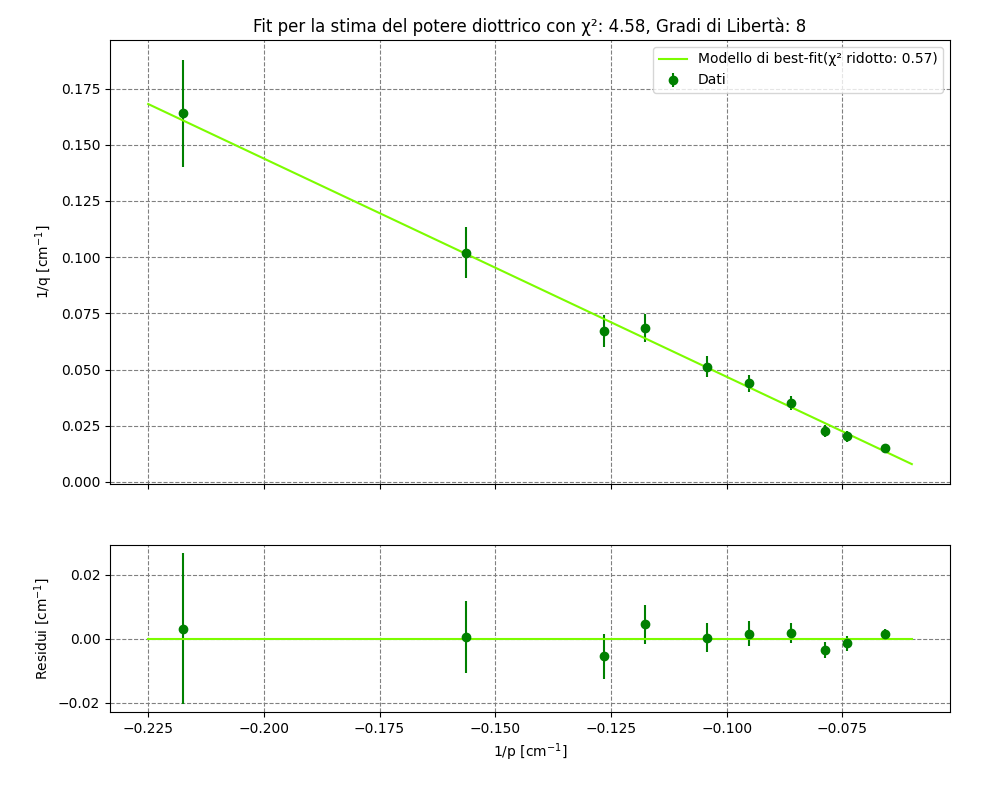
\includegraphics[width=\linewidth]{fit e residui per il potere diottrico.png}
\caption{Fit e residui per il potere diottrico}
\label{fig:f.d}
\end{minipage}
\hfill
\begin{minipage}{0.40\textwidth}
Nella \textbf{Figura~\ref{fig:f.d}} abbiamo il grafico superiore che mostra i dati sperimentali, indicati dai punti verdi, e la linea di best-fit, in verde chiaro, che rappresenta il modello ottimale secondo il metodo dei minimi quadrati. Il titolo del grafico indica un valore di \( \chi^2 \) di 4.95 e 8 gradi di libertà, suggerendo un buon adattamento del modello ai dati. Il grafico inferiore presenta i residui dell'analisi, ovvero le differenze tra i dati sperimentali e i valori previsti dal modello, che sono contenuti entro un intervallo accettabile. Tuttavia, il \( \chi^2 \) ridotto di 0.62 ci suggerisce che i nostri dati, con il corrispondente errore, si adattano un po' troppo bene al modello, anche se questo valore è molto accentuato, come si può osservare dalle barre d'errore della prima misurazione, molto ampie.
\end{minipage}
\end{figure}

Per valutare l'accordo fra il modello e i dati abbiamo calcolato il $\chi^2$ utilizzando sempre gli errori efficaci:
\begin{equation}
\chi^2 = \sum_{i=1}^n \frac{(y_i - f(x_i; \hat{\theta}_1, \ldots, \hat{\theta}_n))^2}{\sigma_{y_i}^2 + \left(\frac{df}{dx}(x_i; \hat{\theta}_1, \ldots, \hat{\theta}_n)\right)^2 \sigma_{x_i}^2}
\end{equation}

\pagebreak
%-------------------------------------------------------------------------------------------------
%---------------------------------------------------------------------------------------------------------------------------------------------------------------------------------------------------------------------------------------------------------------------
\section{Conclusioni}

Questa esperienza ha portato a risultati soddisfacenti. La maggiore difficoltà incontrata è stata quella di determinare con precisione quando l'immagine sullo schermo fosse perfettamente a fuoco, dato che non vi era un punto di messa a fuoco netto ma piuttosto un intervallo in cui l'immagine appariva sufficientemente nitida. 

L'analisi statistica dei dati ha restituito un valore di $\chi^2$ ridotto pari a 0.62, indicando un buon accordo con il modello lineare utilizzato. Tuttavia, questo valore relativamente basso suggerisce che gli errori associati alle misure potrebbero essere stati sovrastimati. Nell'analisi abbiamo assunto che l'errore fosse uniformemente distribuito nell'intervallo di misurazione, data la natura ripetitiva della misura. In futuro, potrebbe essere utile indagare metodi più accurati per la stima degli errori associati a questo tipo di misura.

Nonostante queste piccole perplessità riguardanti la stima degli errori, i dati ottenuti appaiono affidabili e non vi sono motivi per rigettare il modello lineare utilizzato per l'analisi. Nel complesso, l'esperienza ha permesso di determinare con successo la focale della lente divergente in esame.




\pagebreak
\end{document}